\documentclass{article}
\usepackage[ampersand]{easylist}
\usepackage{amsmath}
\usepackage{graphicx}
\graphicspath{ {C:/Users/ustjo/Desktop/Investing/Stocks/canslim/weeklyStockScanner/Trades/figures/} }
\usepackage[inline]{enumitem}
\usepackage{lscape}
\begin{document}
\title{Trade Summary  \\ Symbol: THO \\ 20170906-20171003}
\author{KAI YIN, CHAN}
\maketitle
\section{Trade details}
During 27 days holding period, price reached 129 profit target from 111.5, resulting in 156.79 realised profit (subtracted commissions).

% Table generated by Excel2LaTeX from sheet 'Sheet1'
\begin{table}[htbp]
  \centering
  \caption{Trade details}
    \begin{tabular}{p{5.145em}rrrr}
    \textbf{Date/Time} & \multicolumn{1}{p{4.215em}}{\textbf{Quantity}} & \multicolumn{1}{p{4.215em}}{\textbf{T. Price}} & \multicolumn{1}{p{4.215em}}{\textbf{Proceeds}} & \multicolumn{1}{p{4.215em}}{\textbf{Comm/Fee}} \\
    2017-09-06, 09:30:02 & 9     & 111.5 & -1,003.50 & -0.34 \\
    2017-10-03, 09:31:36 & -9    & 129   & 1,161.00 & -0.37 \\
    \end{tabular}%
  \label{tab:addlabel}%
\end{table}%
\section{Equity curve}
\begin{figure}
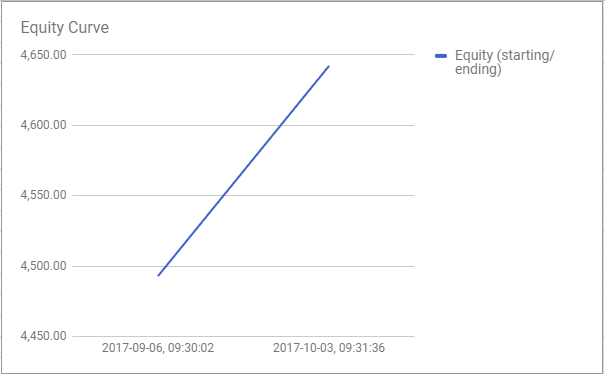
\includegraphics[width=\textwidth,keepaspectratio]{20170906-20171003_THO.PNG}
\end{figure}

\section{Analysis}
\subsection{Performance comparison with SPX}
Within the 27 days holding period, THO return calculated by closing price is 13.3\% and SPX return is 2.93\%

\begin{figure}
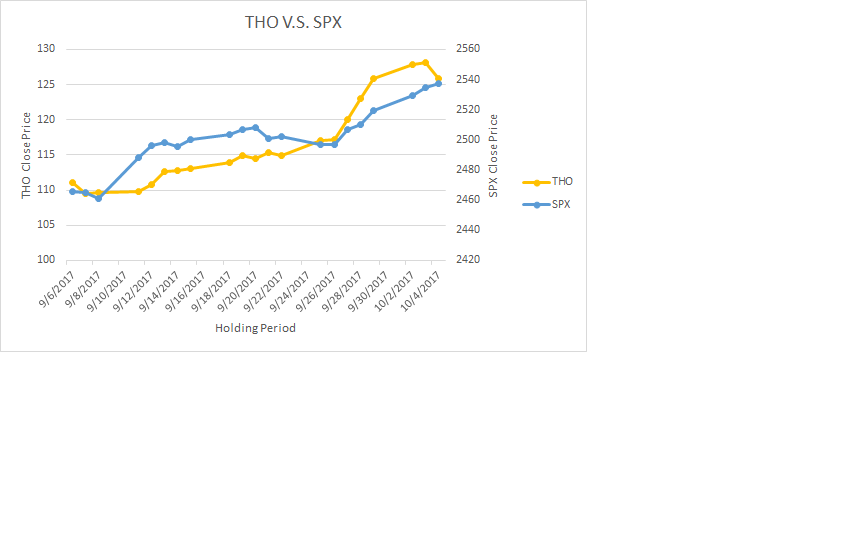
\includegraphics[width=\paperwidth,keepaspectratio] {20170906-20171003_THOSPX.PNG}
\end{figure}
\subsection{Maximum drawdown within investment period}
The maximum drawdown is 2.57\%

\begin{figure}
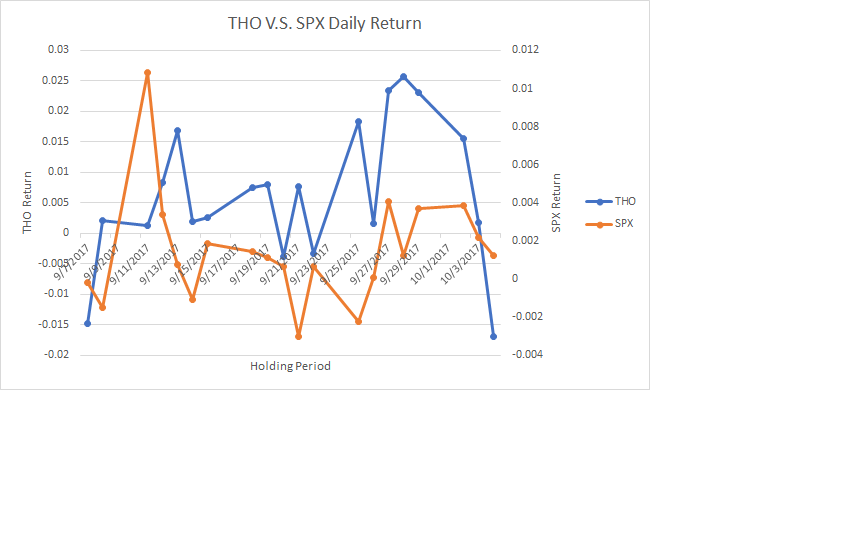
\includegraphics[width=\paperwidth,keepaspectratio]{20170906-20171003_dailyreturn.PNG}
\end{figure}
\end{document}